% !TeX spellcheck = en_US

\chapter{Image Segmentation with Convolutional Neural Networks (CNN)}\label{chp:segmentation_with_neural_networks}
\section{Introduction}
With the increasing computational power that comes with recent graphic cards, increasingly complex neural networks can be used on increasingly challenging tasks. Especially the area of image processing, deep learning gains in popularity. Not only due to the great availability of data sets but also because companies recognize the amount of knowledge and information that can be retrieved with such technologies.

The following sections are a brief introduction into image segmentation using convolutional neural networks.

\section{Object detection and segmentation}
Object detection exists since long before deep learning was so popular as it is now. In object detection, the goal is to determine whether an object of a specified class (for example 'car') is present on an image. Another type of object detection is with additional classification, which means to find all objects on an image together with their class and a probability that the object is actually belongs to the determined class. \autoref{fig:neural_networks:object_detection} shows an example of object detection and classification.

\begin{figure}[H]
    \centering
	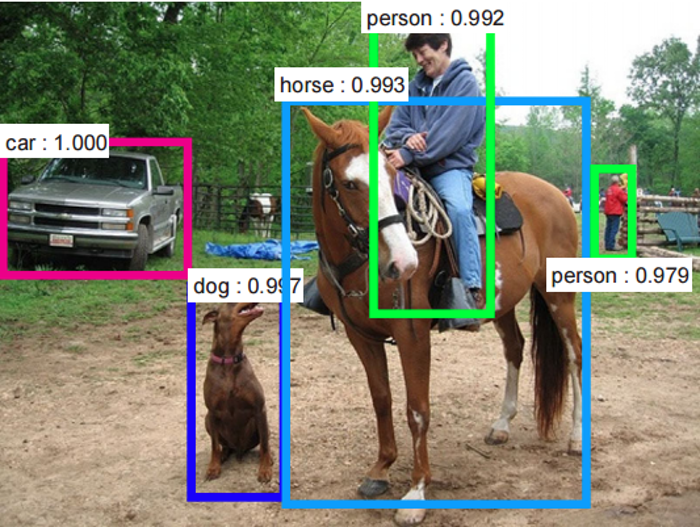
\includegraphics[width=0.6\linewidth]{chapters/neural_networks/images/object_detection.png}
	\caption{An example of object detection, showing the detected classes and the confidence of each prediction.\\ Source: https://dius.com.au/2016/12/06/the-cleverness-of-deep-learning/ (27.05.2018)}
	\label{fig:neural_networks:object_detection}
\end{figure}

In contrast to object detection, the target of image segmentation is not only to state whether an object is present on the image, but to label each pixel of the image with a class, such as 'car' or 'building'. The Different types of image segmentation can be seen in \autoref{fig:neural_networks:image_segmentation}.

\begin{figure}[H]
    \centering
	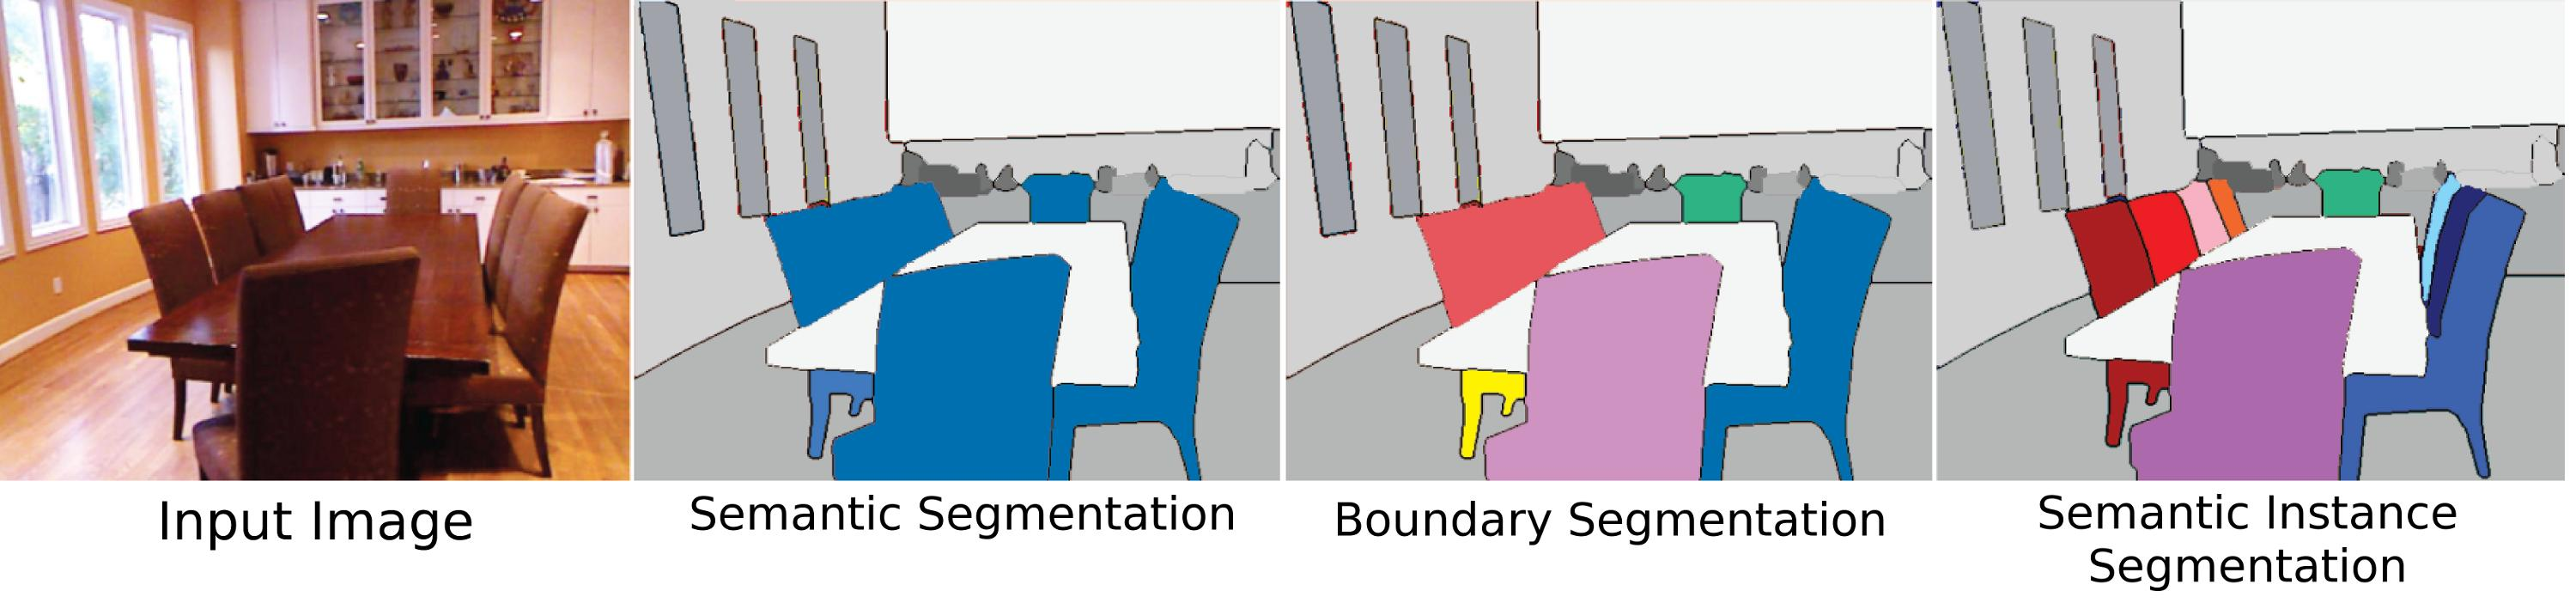
\includegraphics[width=0.8\linewidth]{chapters/neural_networks/images/segmentation.jpg}
	\caption{Different types of image segmentation.\\ Source: https://i.stack.imgur.com/mPFUo.jpg (27.05.2018)}
	\label{fig:neural_networks:image_segmentation}
\end{figure}

\section{Convolutional Layer}
A convolutional layer is one of the most important and basic building blocks of a neural network. It has a number of filters, each of which is small, compared to the input volume (the image), for example 5x5x3 pixels (a 5x5 filter with 3 channels, because standard images have 3 color channels). During the forward pass of the network, the filters are being moved over the input image and at each position of the filters on the image, a convolution is being computed, which is an element wise matrix multiplication and a sum over the resulting matrix. The result of this operation is an activation map, which is also the output of the convolutional layer.

\begin{figure}[H]
    \centering
	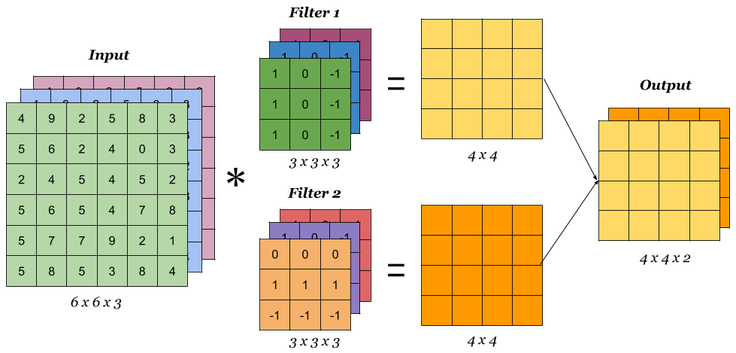
\includegraphics[width=0.8\linewidth]{chapters/neural_networks/images/convolution-with-multiple-filters.png}
	\caption{Convolution with multiple filters\\ Source: https://idoml.com (03.06.2018)}
	\label{fig:neural_networks:convolution_with_multiple_filters}
\end{figure}

Obviously, the size of a filter can be configured, as well as the step size, the stride, and the amount of zero padding around the input image.

\begin{figure}[H]
    \centering
	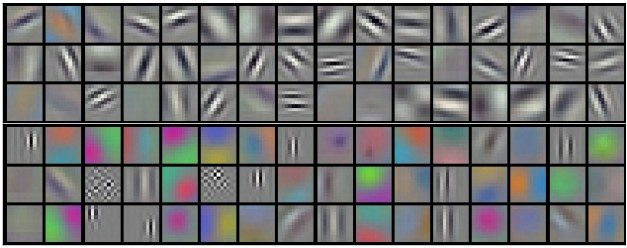
\includegraphics[width=0.6\linewidth]{chapters/neural_networks/images/example_filters.jpeg}
	\caption{Example filters learned by \cite{Krizhevsky.2012}.\\ Source: http://cs231n.github.io/assets/cnn/weights.jpeg (27.05.2018)}
	\label{fig:neural_networks:example_filters}
\end{figure}

\section{Pooling Layer}
Pooling is a technique which allows to reduce the size of an image by extracting a single value from a region of values. The extracted value depends on the pooling type that is used. The most common pooling types are max pooling for extracting the highest value from the current field and average (avg) pooling which extracts the lowest value.

A pooling layer has basically trhee parameters, it can be configured with. Firstly, there is the stride \textit{s} which is the distance the filter is moved. Secondly, there is the filter size \textit{f} which determines the width and height of the filter that is used, to extract the value from the input.

\begin{figure}[H]
    \centering
	\begin{subfigure}{0.4\textwidth}
    	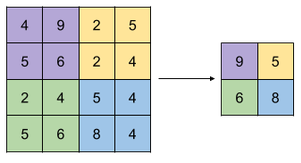
\includegraphics[width=0.9\linewidth]{chapters/neural_networks/images/max_pooling.png}		    \caption{Max Pooling}
    	\label{fig:neural_networks:max_pooling}
	\end{subfigure}~
	\begin{subfigure}{0.4\textwidth}
    	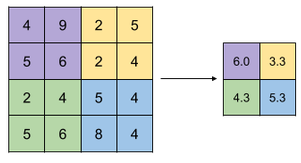
\includegraphics[width=0.9\linewidth]{chapters/neural_networks/images/avg_pooling.png}       	\caption{Average Pooling}
    	\label{fig:neural_networks:avg_pooling}
	\end{subfigure}
	\caption{Max and average pooling\\Source: https://idoml.com (02.06.2018)}
	\label{fig:neural_networks:pooling}
\end{figure}

As described in the previous chapter, a layer can have multiple output channels. Obviously, pooling can also be done with multiple channels, which can be seen in \autoref{fig:neural_networks:max_pooling_multichannel}.

\begin{figure}[H]
    \centering
	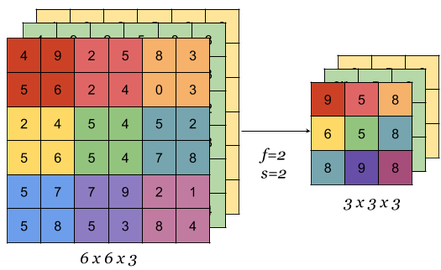
\includegraphics[width=0.6\linewidth]{chapters/neural_networks/images/max_pooling_multichannel.png}
	\caption{Max pooling with multiple channels\\ Source:https://idoml.com (03.06.2018)}
	\label{fig:neural_networks:max_pooling_multichannel}
\end{figure}

\section{Fully Connected Layer}
A fully connected layer is nearly the same as a convolutional layer. The only difference is, that the output of a convolutional layer
is spatially connected only to a region of the previous layer but not to the whole output.
\autoref{fig:neural_networks:fc_and_conv_layer} shows the difference between a fully connected layer and a convolutional layer.


\begin{figure}[H]
    \centering
	\begin{subfigure}{0.4\textwidth}
    	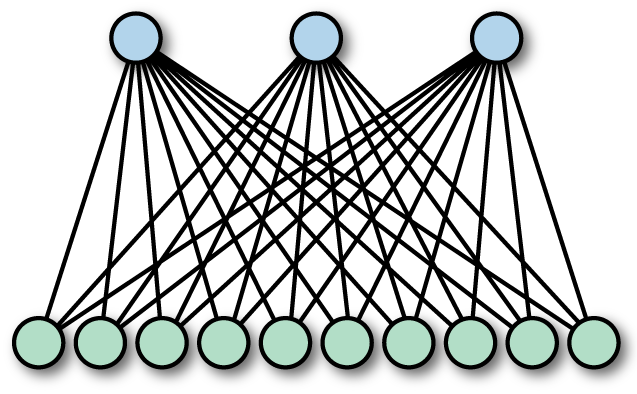
\includegraphics[width=0.9\linewidth]{chapters/neural_networks/images/fc_layer.png}		    \caption{Fully Connected Layer}
    	\label{fig:challenges:max_pooling}
	\end{subfigure}~
	\begin{subfigure}{0.4\textwidth}
    	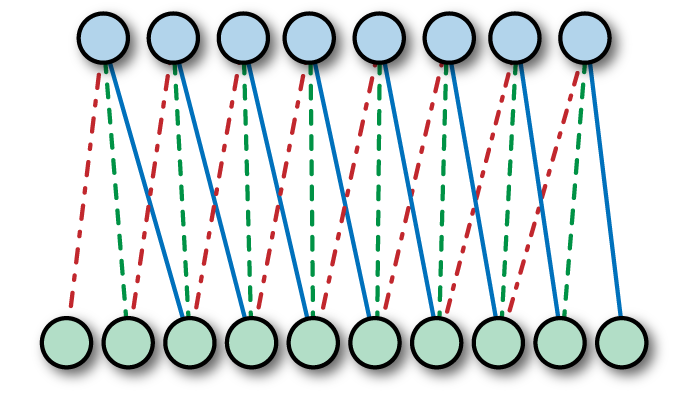
\includegraphics[width=0.9\linewidth]{chapters/neural_networks/images/conv_layer.png}       	\caption{Convolutional Layer}
    	\label{fig:challenges:avg_pooling}
	\end{subfigure}
	\caption{Fully Connected and Convolutional Layers\\Source: https://www.safaribooksonline.com/library/view/learning-tensorflow/9781491978504/ch04.html (07.06.2018)}
	\label{fig:neural_networks:fc_and_conv_layer}
\end{figure}

\section{Mask R-CNN}
Due to the massive amount of research required to come up with or improve an existing state of the art neural network architecture,
this has been out of scope for this work. As a result of this, we decided to use Mask R-CNN \cite{He.20170405} which is, as the name implies, a recurrent, convolutional neural network.